\documentclass{cernatsnote}
\usepackage{siunitx}
\usepackage[table,xcdraw]{xcolor}
%\usepackage[colorinlistoftodos]{todonotes}
\usepackage{placeins}
\usepackage{titlesec}
\usepackage{subfigure}
\usepackage{float}
\usepackage{booktabs}
\setcounter{secnumdepth}{4}
\setcounter{tocdepth}{4}    %
\usepackage{amssymb}
\usepackage{url}

\usepackage{booktabs}
\usepackage{multirow}
\usepackage{rotating,tabularx}

\titleformat{\paragraph}
{\normalfont\normalsize\bfseries}{\theparagraph}{1em}{}
\titlespacing*{\paragraph}
{0pt}{3.25ex plus 1ex minus .2ex}{1.5ex plus .2ex}



%%%%%%%%%%%%%%%% TITLE PAGE %%%%%%%%%%%%%%%% 
    \title{CHIMERA November 2022 Report}
    \author{
    	To be completed \; \\		
    	CERN, CH-1211 Geneva, Switzerland
    }
    \date{\today}
    \keywords{}
    \begin{document}
    \newcommand{\figref}[1]{Fig.\,\ref{#1}}
    \newcommand{\tabref}[1]{Table\,\ref{#1}}
    \newcommand{\secref}[1]{Section\,\ref{#1}}

    \maketitle
    
    \begin{abstract}
        \ldots
    \end{abstract}
%%%%%%%%%%%%%%%% TITLE PAGE END %%%%%%%%%%%% 

    \begingroup
    \color{black}
    \pagebreak
    \tableofcontents
    \endgroup

\pagebreak

\section{Introduction} %all
\begin{figure}[!htb]
\centering
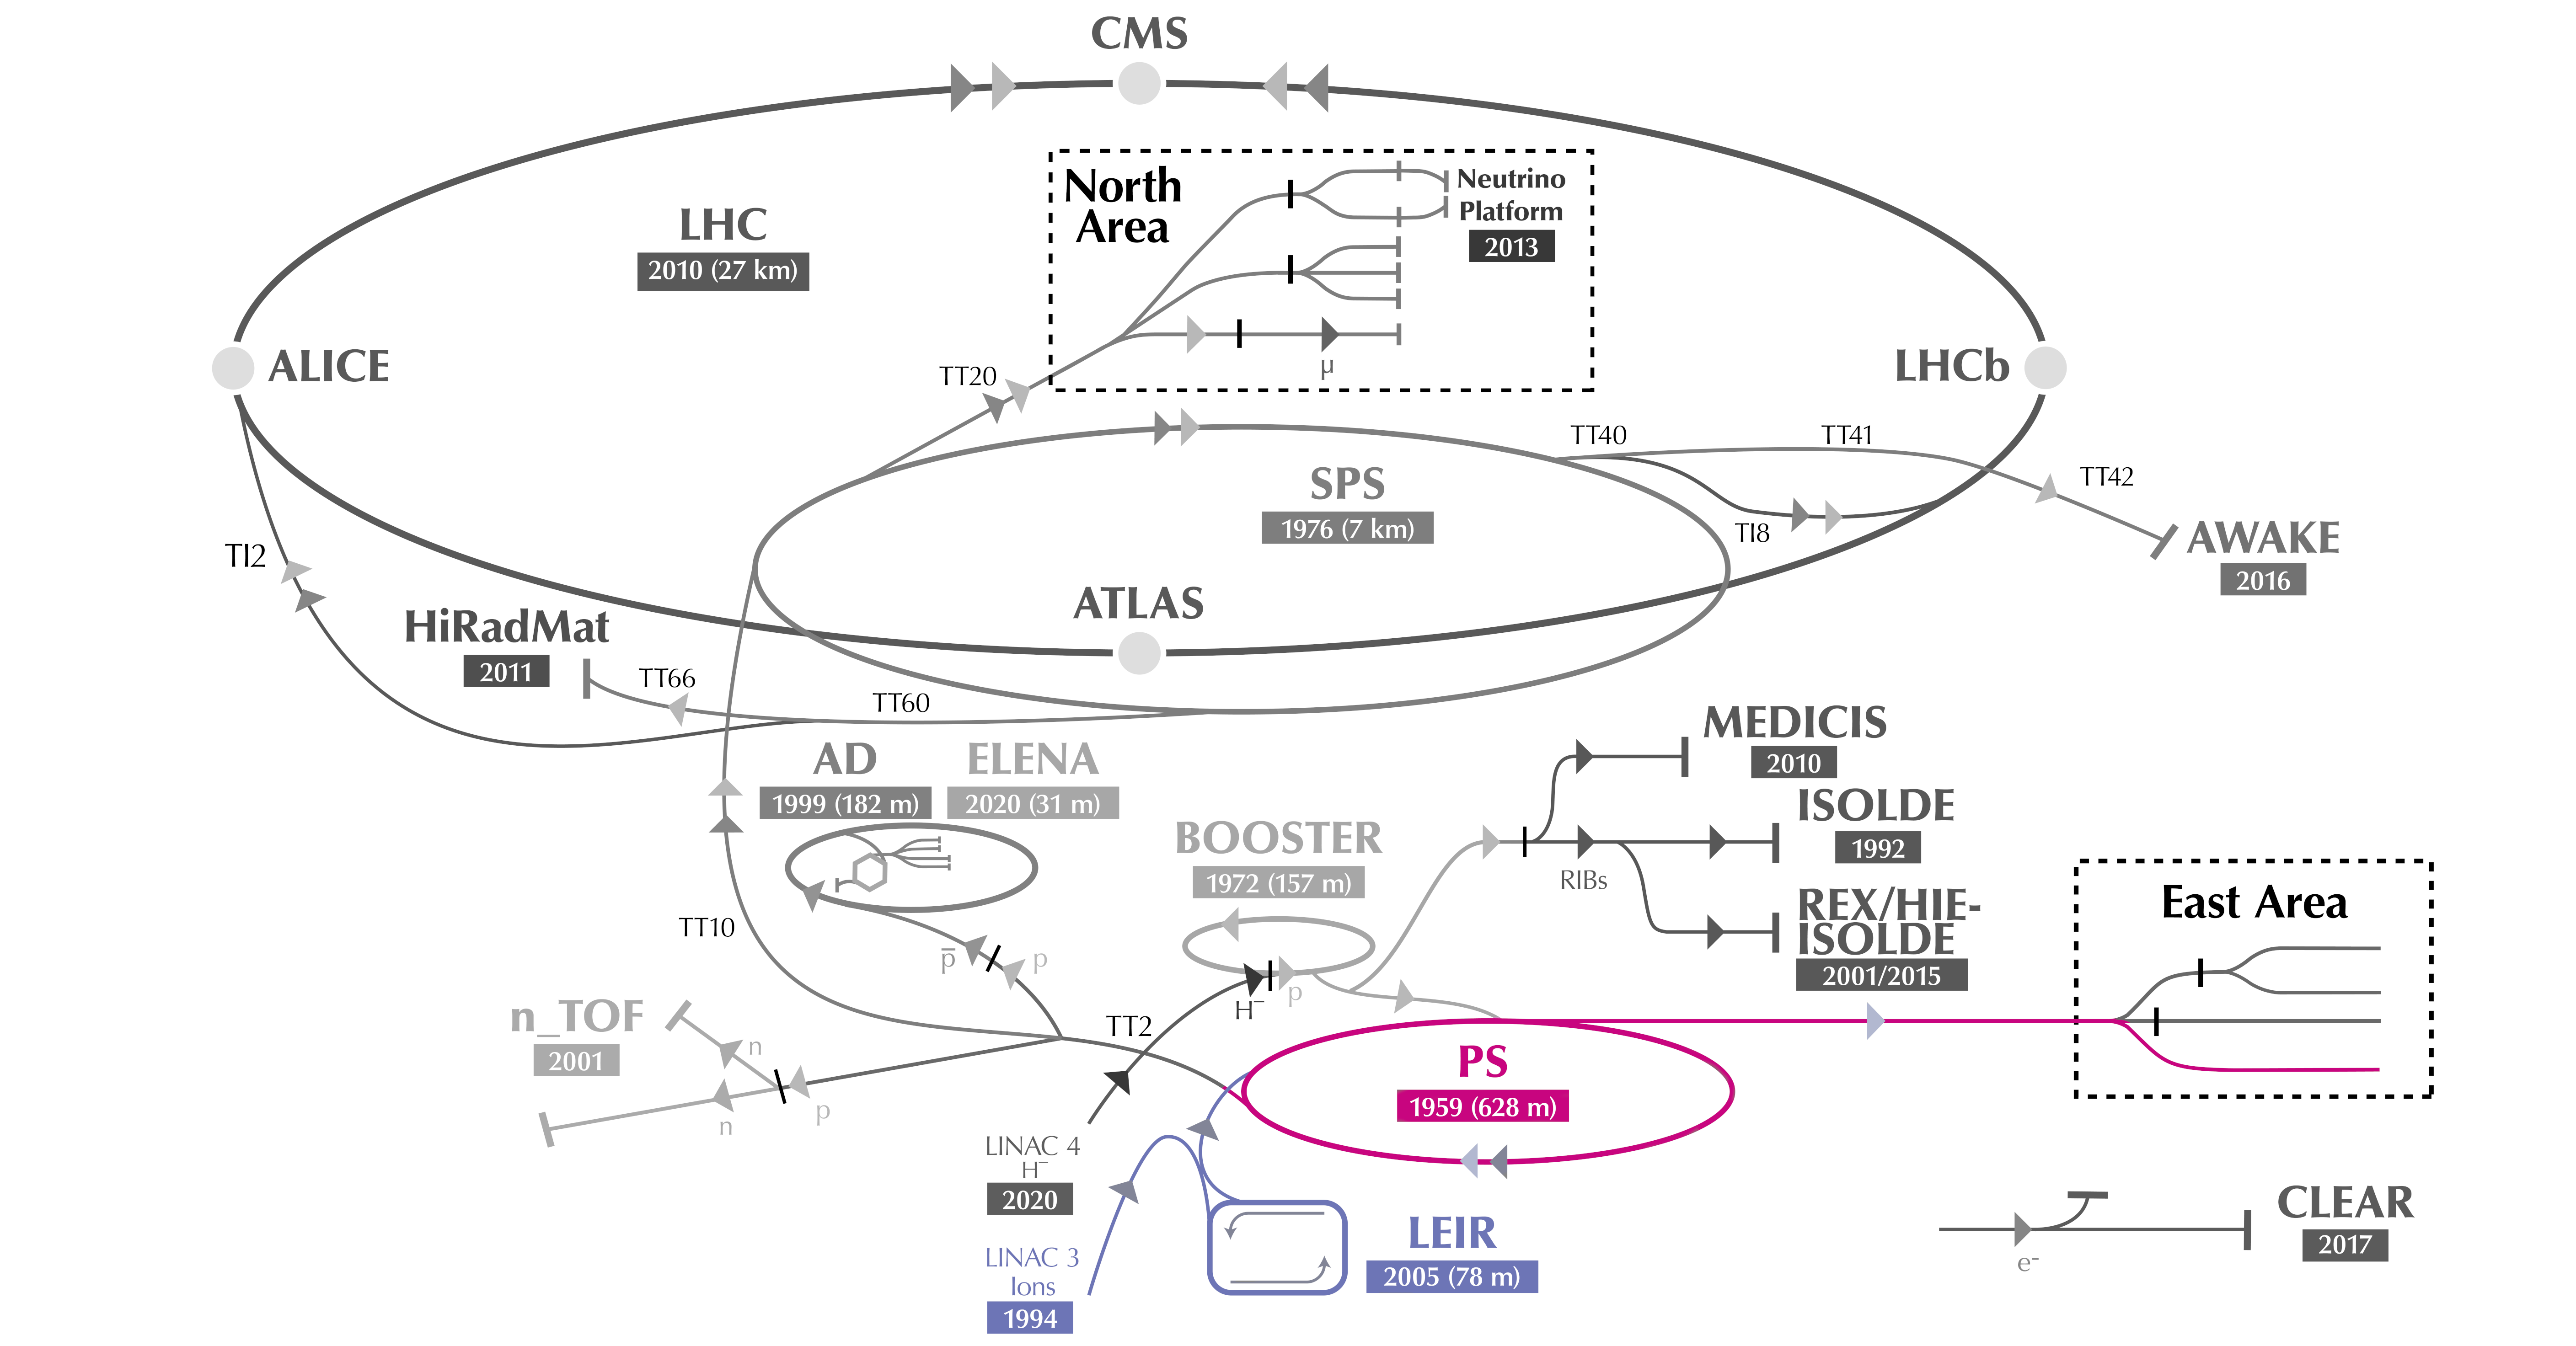
\includegraphics[width=1.0\textwidth]{images/CCC_eastt8_small.png}
\caption{The CERN accelerator complex. The lead ion beam used by CHIMERA is highlighted in color.}
\label{fig:CCC}
\end{figure}

\section{Beam properties - PS configuration and T8 beam instruments}
% as set in the PS and measured by the beam instruments

\subsection{Proton Synchrotron beam energy} % Eliott
% Some intro about how it is defined, including the lookup tables
% The nice colour showing which energy was used during each moment of the test
%Introduction:

%Briefly explain what an accelerator is and its importance in scientific research
The Proton Synchrotron (PS) is part of the injector chain and used to accelerate particles from the Proton Sychrotron Booster (PSB) to the SPS and finally to the Large Hadron Collider (LHC). For the purpose of CHIMERA, it can also be receive and accelerate heavy ions from the Low Energy Ion Ring (LEIR) and extract them to the East Area. The PS uses radio frequency (RF) cavities to accelerate charged particles, such as protons or Pb ions, to high energies and uses 100 dipoles to bend the beam around it's 628 m circumference \cite{}. These particles are then extracted using slow extraction through a beam line and transported to the CHARM facility where the CHIMERA instruments are located.

%Introduce the concept of beam energy and its significance in the operation of an accelerator
Beam energy refers to the kinetic energy per nucleon $E_{kin}$ of the charged particles beam. The relationship for an ion beam is  $E_{kin, TOT}=E_{kin}\cdot A$, where A is the atomic mass number (A=Z+N, number of protons Z and neutrons N). The total momentum for an ion beam is

$$pc={E_{0}\sqrt{\gamma^{2}-1}}$$

$$pc = E_{0}\sqrt{\left [ \left( \frac{E_{kin}}{E_{0}}+1\right )^{2}-1\right ]}$$

where, $E_{0}$ is the rest mass of the ion and $\gamma=\frac{E}{E_{0}}=\frac{E_{0}+E_{cin}}{E_{0}} = \frac{E_{cin}}{E_{0}}+1$

The rigidity is defined as:
$$B\rho = \frac{pc}{q}$$

\subsubsection{CHIMERA beam}

The CHIMERA beam uses a lead ion beam. It is partially stripped during acceleration Pb54+ (which means it has 54 charges and 28 $e^{-}$ remaining) of isotope A=208 of energy 1 GeV per nucleon the momentum would be:

$$pc = E_{0}\sqrt{\left [ \left( \frac{1\text{ [GeV]}\cdot 208}{E_{0}}+1\right )^{2}-1\right ]}$$

where the rest mass $E_{0}$ of Pb54+ is:

$$m_{Pb54+}= 82\cdot m_{proton} + 126\cdot m_{neutron} + 28\cdot m_{e^{-}} - m_{defect} = 193.74 \frac{\text{GeV}}{\text{c}^{2}}$$

with the mass defect: $m_{defect}=82\cdot m_{proton} + 126\cdot m_{neutron} + 28\cdot m_{e^{-}} - 208\cdot m_{u}$ 

$$m_{p} = 0.93828 \text{ } GeV/c^{2}$$
$$m_{n} = 0.93957 \text{ } GeV/c^{2}$$
$$m_{e^{-}} = 0.000511 \text{ } GeV/c^{2}$$
$$m_{u} = 0.9315 \text{ } GeV/c^{2}$$
\cite{boston_university_nuclear_nodate}

\subsection{Example calculation}

$$B\rho \text{ [T m]} = 3.3356\cdot p \text{ [GeV/c]}$$
where for the PS, $\rho = 70.0789$ m.

Figure \ref{fig:bfield} shows the shape of the magnetic field in the main dipoles of the PS produced by POPS. There is the injection plateau, the flat-top and a spike at the end to circumvent some limitation of POPS.

\begin{figure}[h]
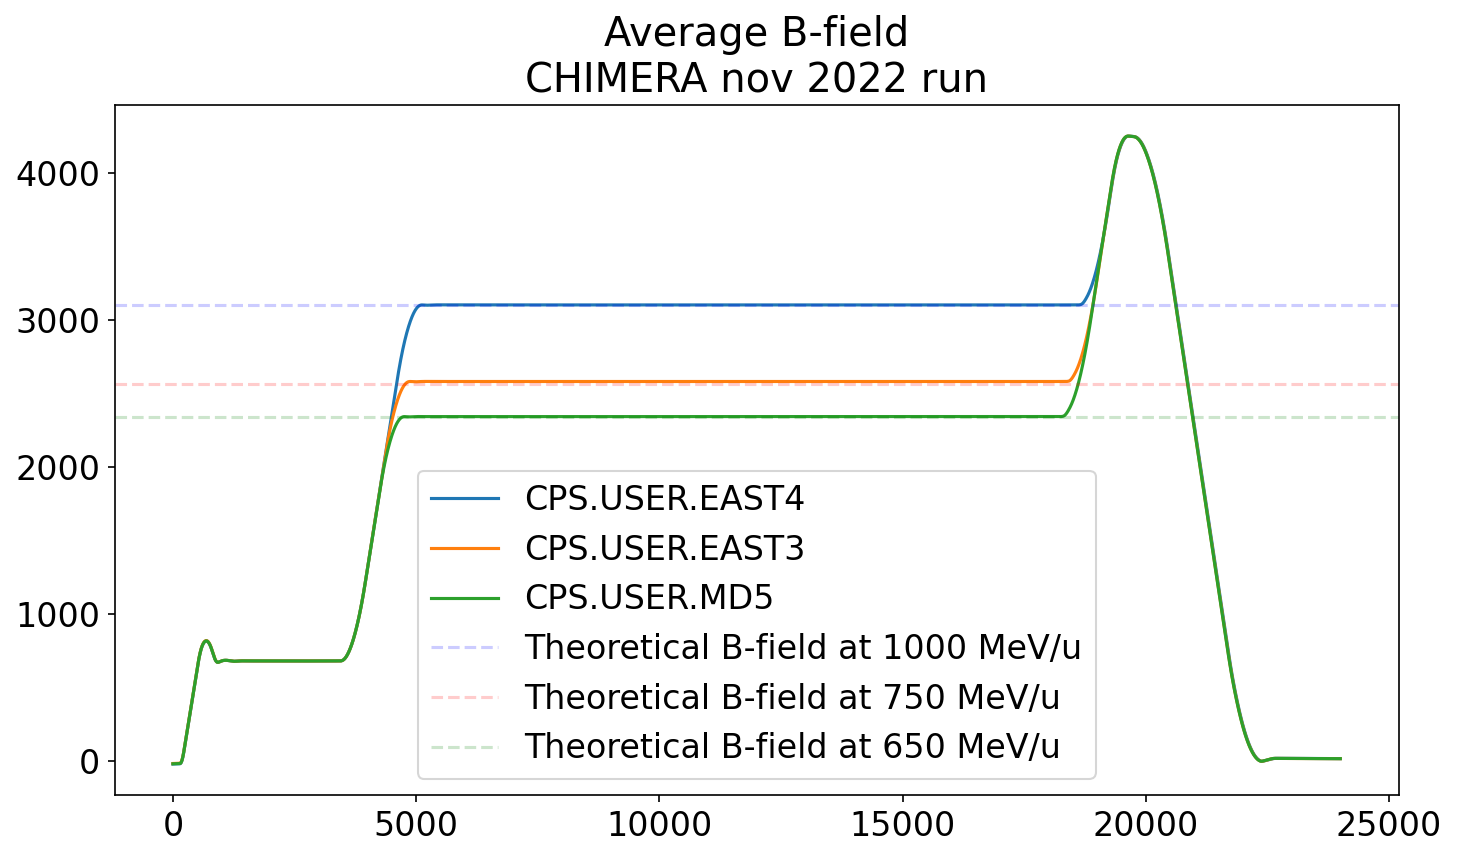
\includegraphics[width=0.9\textwidth]{images/average_b_field_chimera.png}
\caption{CHIMERA B-field for different energies}
\label{fig:bfield}
\end{figure}

\subsubsection{Energy scan}

For development purposes and after the ESA run, we ramped the beam energy using an automatic script.

\begin{figure}[h]
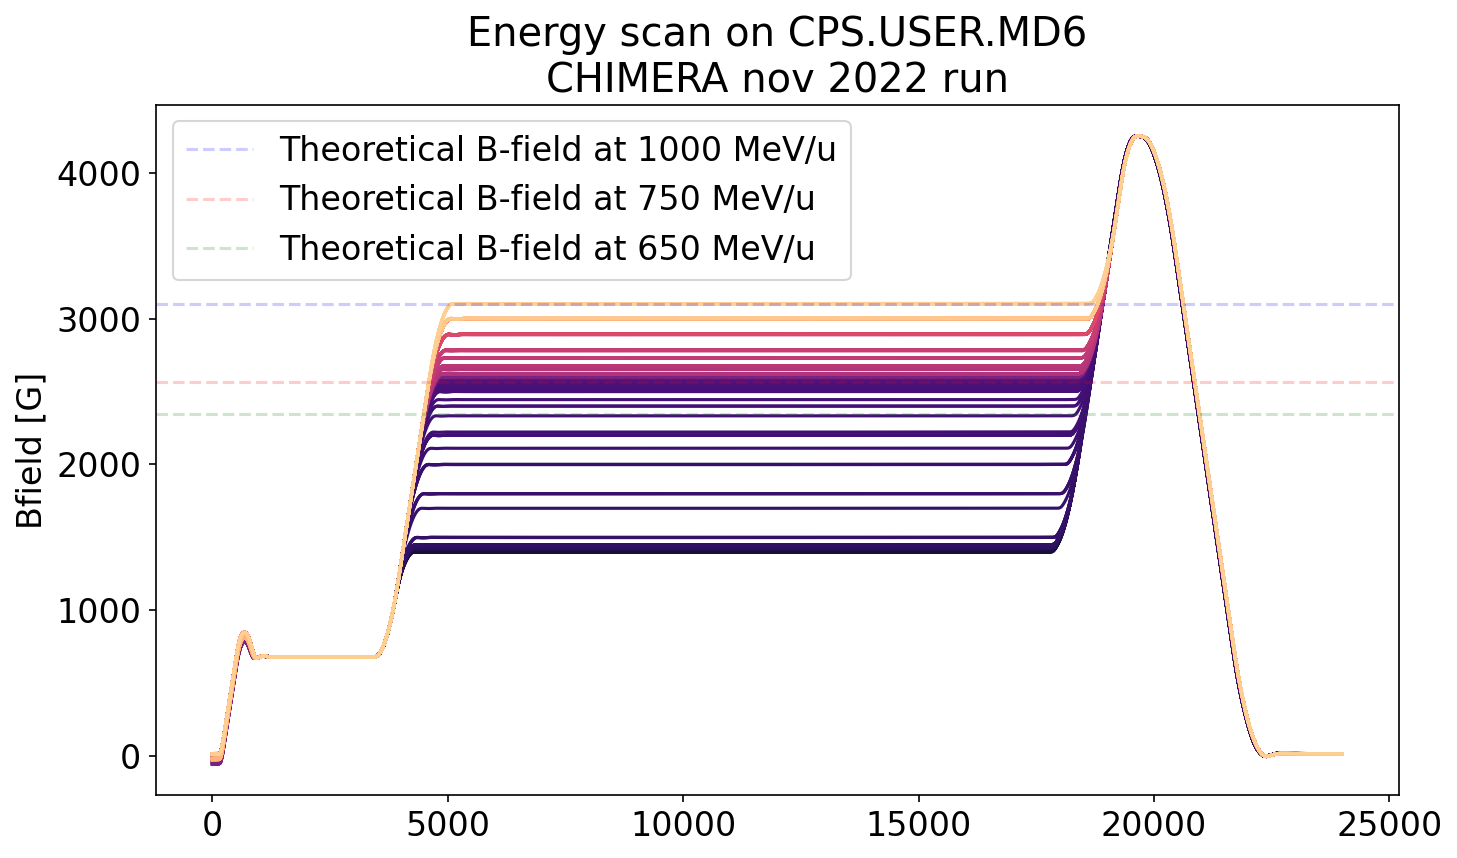
\includegraphics[width=0.9\textwidth]{images/energy_scan_chimera 1.png}
\caption{CHIMERA B-field for different energies}
\label{fig:bfield}
\end{figure}


\begin{figure}[h]
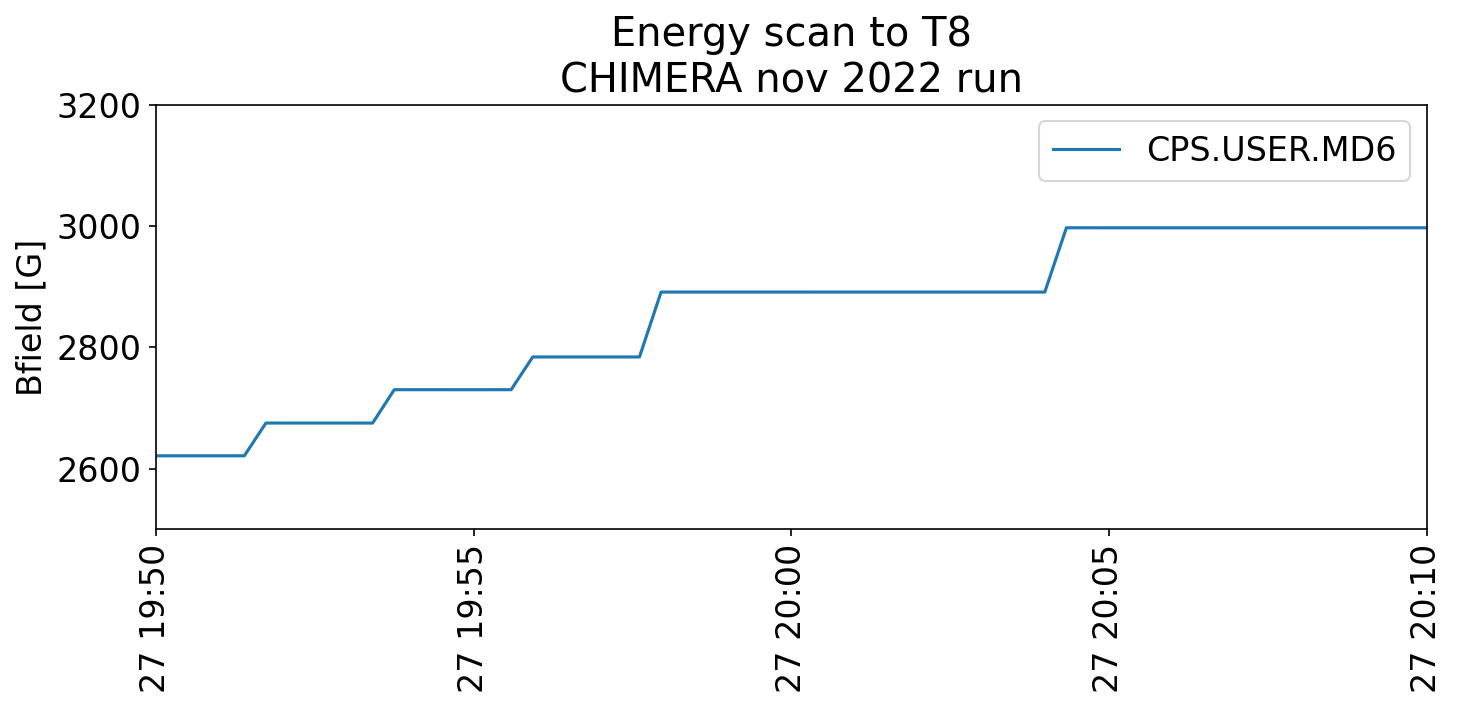
\includegraphics[width=0.9\textwidth]{images/energy_scan_timestamp_chimera 1.png}
\caption{CHIMERA B-field for different energies}
\label{fig:bfield}
\end{figure}


\subsection{Beam intensity} % Eliott, Kacper
% RFKO and gain settings throughout the test
% Intensity measurements on SEC and XION, including intensity vs. gain
The slow extraction of the beam is controlled via the RF-Knock out (RFKO) technique. This allows a precise and reproducible intensity control spill by spill.

An RFKO extraction process involves using a transverse beam disturbance with a noise signal whose frequency changes over time (frequency modulation (FM)). This change in frequency is necessary to affect all particles. We do a sweep - or chirp - in frequency. 

With the noise from the chirp, the particles are diffused from the beam core to the stable triangle.

\begin{figure}[h]
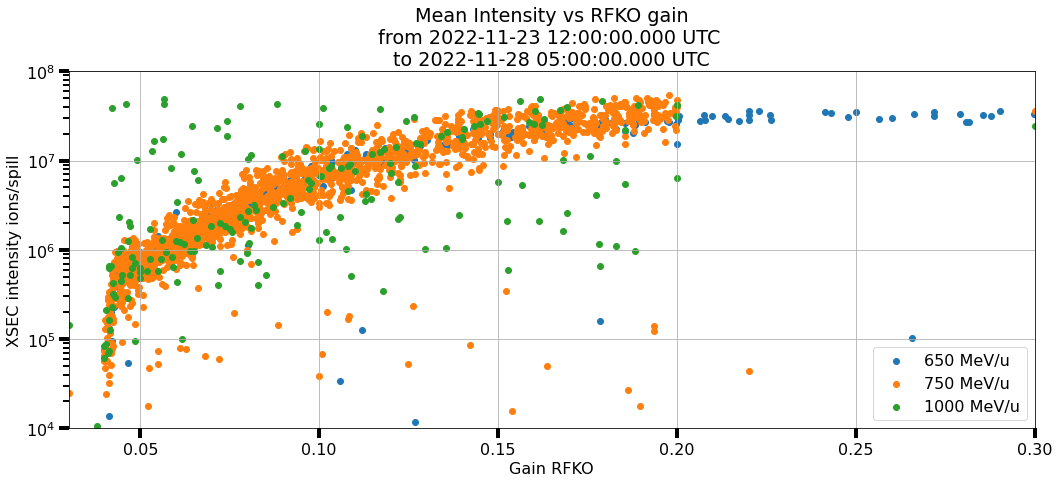
\includegraphics[width=0.9\textwidth]{images/xsec70_intensity_vs_gain.png}
\end{figure}

The RFKO has different parameters to control the extraction:
- Chirp gain: the voltage applied to the RFKO plates.
- Chirp frequency range
- Accuracy (number of turns in the PS)
- Bounds: Start and stop of the chirping

Lowest chirps is 512 turns
Time it takes for one turn in the PS = **2.1 $\mu s$**
* $t = \frac{circumference}{c} = \frac{628}{3e8} = 2.1e-6 [s]$

5.12e2 * 2.1e-6 = 1.752e-3 s = 1.8 ms

\begin{figure}[h]
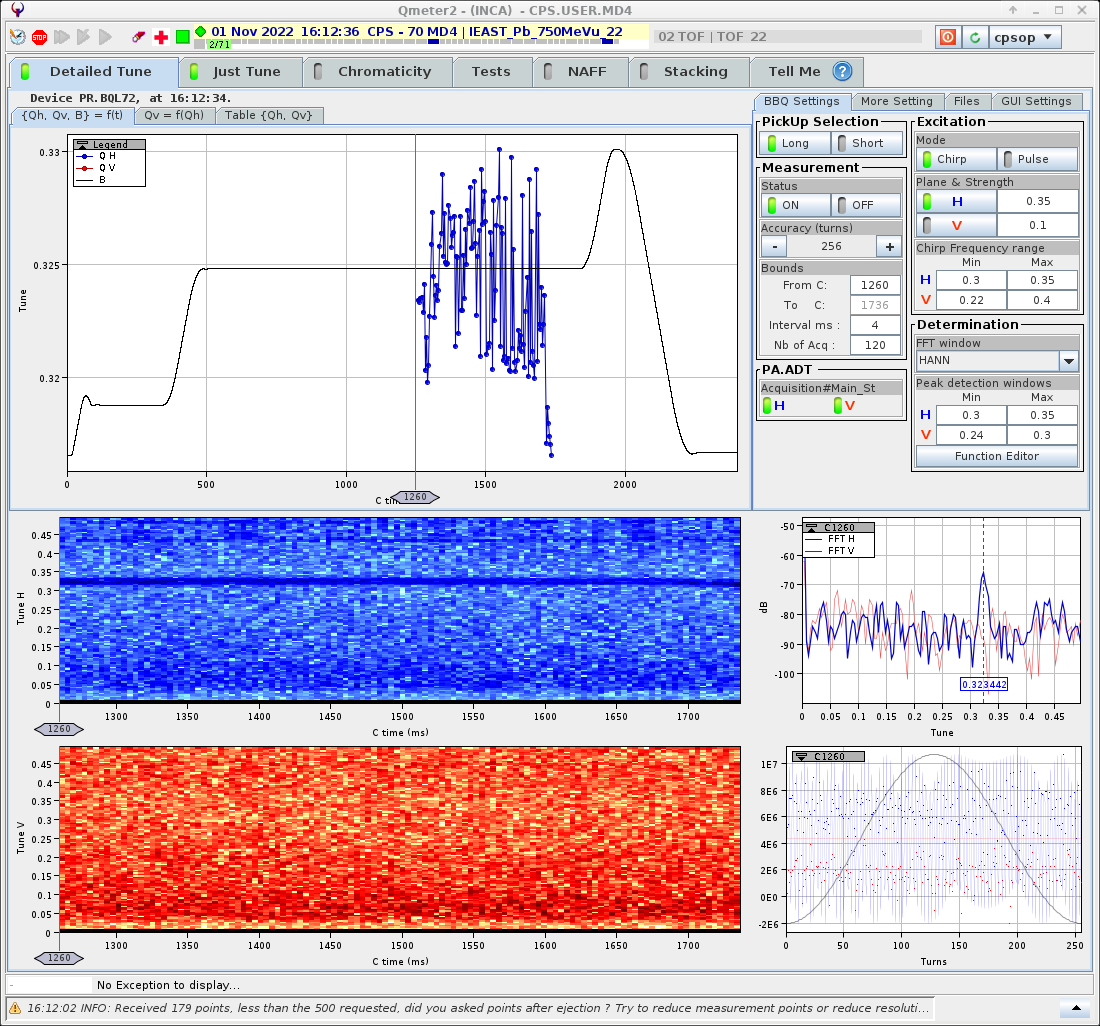
\includegraphics[width=0.4\textwidth]{images/qmeter.png}
\end{figure}

\begin{figure}[h]
\centering
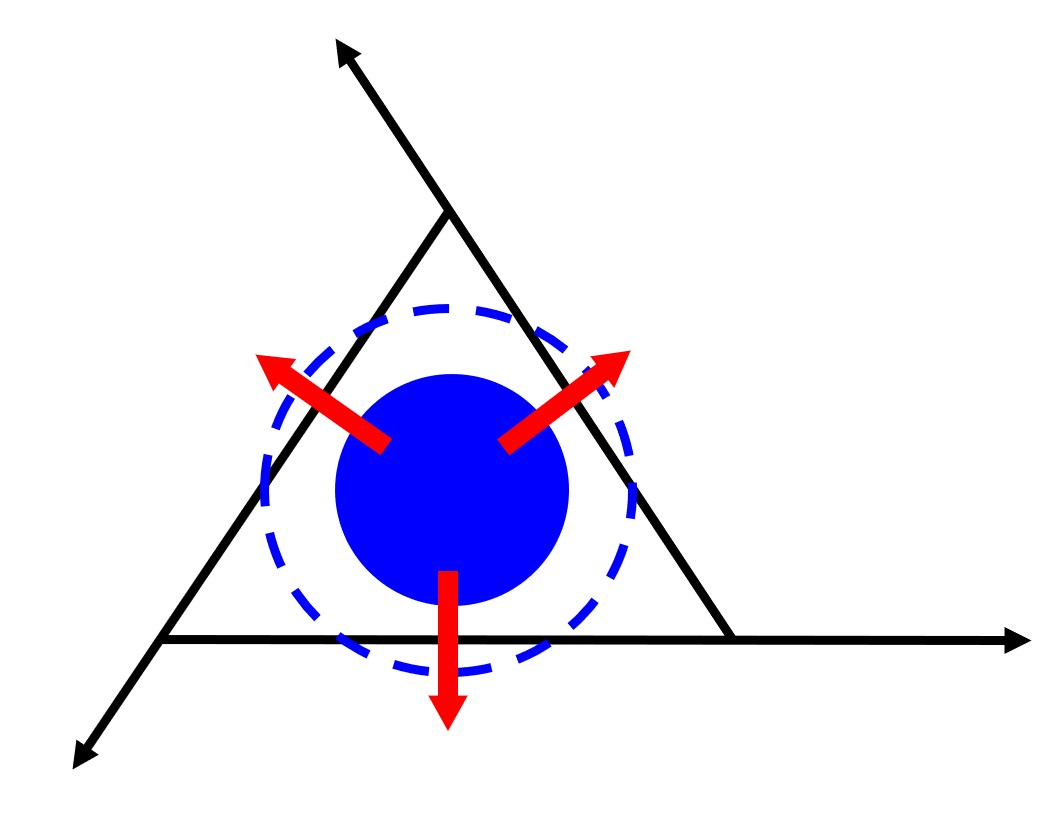
\includegraphics[width=0.4\textwidth]{images/RFKO.jpg}
\end{figure}


\subsection{Spill time profile} % Eliott
% Gas scintillator, SEC, XION, etc.
% Diode SMU measurements could be included here, even if introduced later
An example of the spill time profile is shown in Fig. \ref{fig:spill_time_profile}.

\begin{figure}[!htb]
\centering
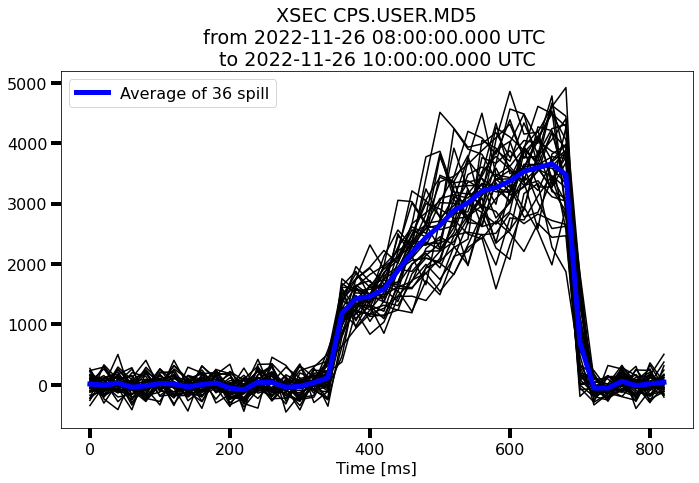
\includegraphics[width=0.6\textwidth]{images/Pasted image 20221130110602.png}
\caption{Spill time profile}
\label{fig:spill_time_profile}
\end{figure}

\subsection{Beam spatial profile} %Eliott, Kacper
% MWPC, Independence of beam profile with beam intensity, impact of energy on the beam shape, “explanation” of the dips (i.e. comparison with and without Montract), etc.
\input{sections/Beam_spatial_profile.tex}

\section{Beam properties - solid state detector in DUT position}
% as measured by the silicon diode

\subsection{Setup} % Natalia
% Montrac, cabling, x-y table, degraders/collimators, etc.
\input{sections/Setup.tex}

\subsection{Diode as a flux monitor} % Kacper
% Including notably the correlation with SEC and XION
\input{sections/Diode_as_flux_monitor.tex}

\subsection{Energy deposition distributions} % Andreas, Natalia
% « Primary » energies, including mysterious energy changes
% Comparison with GSI, which we can consider as calibration/reference
% Impact of degraders
% Impact of collimation
\input{sections/Energy_deposition_distributions.tex}

\section{Other measurements}
\subsection{SRAM memories} % Andrea
% SEU counts versus beam intensity
% (note: for actual SEU cross section value/fluence measurements, we would need to accurately know the beam LET, which will in turn likely need to at least partially rely on a combination of simulations and diode measurements. But, we can try to, in first instance, focus on the diode measurements – also because these mysterious energy changes cannot be accounted for in FLUKA, unless understood)
\input{sections/SRAM_memories.tex}

\subsection{Scintillator} % Andreas
\input{sections/Scintillator.tex}

\newpage
\bibliography{references, references_eliott}
\bibliographystyle{IEEEtran}

\end{document}